\section{Introduction}
Unlike other systems, in distributed systems developers have to face additional challenges, such as concurrency,
asynchrony, and partial failure while tracing a buggy execution, which require them to consider all possible ways that non-determinism might manifest itself. Since the number of event orderings a distributed system may encounter grows exponentially with the number of events, bugs are commonplace.

Software developers commonly discover anticipated bugs through unit and integration tests. To uncover unanticipated cases, semi-automated testing techniques such as fuzzing (where sequences of message deliveries, failures, etc. are injected into the system) are effective. The system can run for long periods and if a problem manifests, then the resulting executions can contain a large number of events, most of which are not relevant to triggering the bug. Understanding how a trace containing thousands of concurrent events lead the system to an unsafe state requires significant expertise, time and luck.

Faulty execution traces can be made easier to understand if they are first minimized, so that only events that
are relevant to triggering the bug remain. Automated minimization tools for sequential test cases \cite{1,2} have already proven themselves valuable, and are routinely applied to bug reports for software projects such as Firefox, LLVM, and GCC.


In this paper, the problem of automatically minimizing executions of distributed systems is addressed and also  focused on executions generated by fuzz testing. Distributed executions have two distinguishing features. Most importantly, input events (e.g., failures) are interleaved with internal events (e.g., intra-process message deliveries) of concurrent processes. Minimization algorithms must therefore consider both which input events and which event schedules are likely to still trigger the bug.

In \cite{3}, STS has been  proposed to minimize the execution for retriggering a bug without analyzing the code. It targeted a specific distributed system (SDN controllers), and focused on minimizing input events given limited control over the execution. In this paper, Distributed Execution Minimizer (DEMi) will be discussed elaborately, which exercises significantly greater control, employs new minimization strategies that quickly reduce the input events, external events, message contents.

The rest of the paper is organized as follows. In Section-I, we will discuss on the basics of the distributed system model and we will define the problem statement. In Section-III, how the DEMi works will be explained. In Section-IV, we will present some of significant minimization results that is found. In Section-V, the current limitations of the tool will be given. Finally, conclusions and future work possibility will be discussed in Section-VI.


\section{Problem Statement}
At the beginning, a model of distributed systems is introduced as groundwork for defining the goals. It has been  believed this model is general enough to capture the behavior of many practical systems.

\subsection{System Model}
Following \cite{4}, a distributed system is modeled as a collection of N single-threaded processes communicating
through messages. Each process $p$ has unbounded memory, and behaves deterministically according to a transition function of its current state and the messages it receives. The overall system $S$ is defined by the transition
function and initial configuration for each process. The graphical view of the overall system is depicted in Figure \ref{system}.

Processes communicate by sending messages over a network. A message is a pair $(p,m)$, where $p$ is the identity of the destination process, and $m$ is the message value. The network maintains a buffer of pending messages that have been sent but not yet delivered. $Timers$ are modeled as messages a process can request to be delivered to itself at a specified later point in the execution.

A $configuration$ of the system consists of the internal state of each process and the contents of the network's
buffer. Initially the network buffer is empty.

\begin{figure}[!t]
\centering
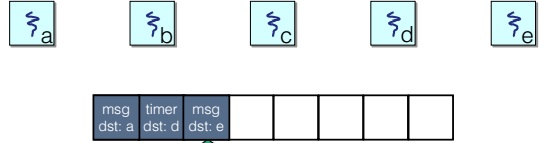
\includegraphics[width=2.5in]{./image/system.png}
\caption{Distributed System Model.}
\label{system}
\setlength{\belowcaptionskip}{-3pt}
\end{figure}

An event moves the system from one configuration to another. Events can be one of two kinds. $Internal$ events
take place by removing a message $m$ from the network's buffer and delivering it to the destination $p$. Then, depending on $m$ and $p$'s internal state, $p$ enters a new internal state determined by its transition function, and sends a finite set of messages to other processes. Since processes are deterministic, internal transitions are completely determined by the contents of $m$ and $p$'s state.

Events can also be $external$. The three external events we consider are: process starts, which create a new process; forced restarts (crash-recoveries), which force a process to its initial state; and external message sends $(p,m)$, which insert a message sent from outside the system into the network buffer (which may be delivered later as an internal event).

A $schedule$ is a finite sequence $\tau$ of events (both external and internal) that can be applied, in turn, starting from an initial configuration. Applying each event in the schedule results in an execution.

\subsection{Testing}
An invariant is a predicate $P$ (a safety condition) over the internal state of all processes at a particular configuration $C$. A configuration $C$ violates the invariant if $P(C)$ is $false$, denoted as $\bar{P}(C)$. A test orchestrator generates sequences of external events $E = $$[e_1,e_2,...,e_n]$, executes them along with some (arbitrary) schedule of internal events, and checks whether any invariants were violated during the execution. The test orchestrator records the external events it injected, the violation it found, and the interleavings of internal events that appeared during the execution.

\subsection{Problem Definition}
We are given a schedule $\tau$ injected by a test orchestrator along with a specific invariant violation $\bar{P}$ observed at the end of the test orchestrator’s execution.

The main goal is to find a schedule containing a small sequence of external (input) events that reproduces the
violation $\bar{P}$. Formally, a $minimal$ $causal$ $sequence$ $(MCS)$ to be a subsequence of external events
$\acute{E} \sqsubseteq  E$ is defined such that there exists a schedule containing $\acute{E}$ that produces $\bar{P}$.

\section{The Proposed Approach}
The proposed approach starts by minimizing external (input) events because they are the first level of abstraction that developers care about. For more difficult bugs, developers typically step through the internal events of the execution to understand  more precisely how the system arrived at the unsafe state. To help with these cases, DEMi turns to minimizing internal events after the external events have been minimized. At this stage, it fixes the external events and search for smaller schedules that still triggers the invariant violation, for example, by keeping some messages pending rather than delivering them. Lastly, it seek to minimize the contents (e.g. data payloads) of external messages.

Conceptually, trivial way to  find MCSes by enumerating and executing every possible schedule containing the given external events. The globally minimal MCS would then be the shortest sequence containing the fewest external events that causes the safety violation. Unfortunately, the space of all schedules is exponentially large, so executing all possible schedules is not feasible.

To find MCSes in reasonable time, DEMi splits schedule exploration into two parts. It starts by using delta debugging \cite{5}, a minimization algorithm similar to binary search, to prune extraneous external events. Delta debugging works by picking subsequences of external events, and checking whether it is possible to trigger the violation with just those external events starting from the initial configuration. The system assumes that a time budget is given by the user, and the system spreads this budget evenly across each subsequence's exploration. DEMi uses Dynamic Partial Order Reduction (DPOR) to prune the schedule space generated from different sequence of internal events by eliminating equivalent schedules then it prioritizes the order in which the exploration of the schedule space to search for MCSes would produce faster exploration.

Thus, the overall strategy is to (i) pick subsequences with delta debugging, (ii) explore the execution of that subsequence with a modified version of DPOR, starting with a schedule that closely matches the original, and then by exploring nearby schedules, and (iii) once a near-minimal MCS is found, it attempts to minimize the number of internal events. With this road map in mind, below the minimization approach is illustrated in greater detail.

\subsection{Choosing Subsequences of External Events}
The task of minimizing a sequence of external events E is modeled such that, that causes an invariant violation as a function ExtMin that repeatedly removes parts of E and invokes an oracle to check whether the resulting subsequence, $\acute{E}$, still triggers the violation. If $\acute{E}$ triggers the violation, then it can be assumed that the parts of E removed to produce $\acute{E}$ are not required for producing the violation and are thus not a part of the MCS. However, this would require that it needs to check $O(|E|)$ subsequences. For minimizing, DEMi therefore applies delta debugging \cite{6}, an algorithm similar to binary search, to achieve $O(log(|E|))$ average case runtime.

\subsection{Checking External Event Subsequences}
Since the number of possible schedules is exponential in the number of events for a subsequence of external events generated by delta debugging, pruning this schedule space is essential to finishing in a timely manner. As others have observed \cite{7}, many events occurring in a schedule are commutative, i.e., the system arrives at the same configuration regardless of the order events are applied. For example, consider two events $e_1$ and $e_2$, where $e_1$ is a message from process a being delivered to process $c$, and $e_2$ is a message from process $b$ being
delivered to process $d$. Assume that both $e_1$ and $e_2$ are co-enabled, meaning they are both pending at the same
time and can be executed in either order. Since the events affect a disjoint set of nodes ($e_1$ changes the state at $c$, while $e_2$ changes the state at $d$), executing $e_1$ before $e_2$ causes the system to arrive at the same state it would arrive at if we had instead executed $e_2$ before $e_1$. $e_1$ and $e_2$ are therefore commutative. Dynamic Partial Ordering Reduction (DPOR)\cite{8} is a well-studied technique for pruning commutative schedules from the search space.

For exploring the schedules DPOR  picks a pending message to deliver, dynamically computes which other pending events are not concurrent with the message it just delivered, and sets backtrack points for each of these, which it will later use (when exploring other non-equivalent schedules) to try delivering the pending messages in place of the message that was just delivered. For maximizing the probability that invariant violations are discovered
quickly while exploring a fixed number of schedules, we employ a set of schedule exploration strategies to guide
DPOR’s exploration, which we describe next.

\subsection{Schedule Exploration Strategies}
This scheduling strategy implements a backtrack prioritization order. Scheduling strategies return the first
violation-reproducing schedule they find (if any) within their time budget. The following observations are considered while exploring schedules:

\textbf{Observation \#1: Stay close to the original execution.}
The original schedule is the main 'guide' for how the system can lead to the same unsafe state. Modified schedules that have causal structures that are close to the original schedule have been chosen. A single, uniquely defined schedule for each external event subsequence is considered and then delivers only messages whose source,
destination, and contents match those in the original execution, in the exact same
order that they appeared in the original execution. If an internal message from the original execution is not pending at the point that internal message should be delivered, it is skipped and move to the next message from the original execution. Similarly, if any pending messages that do not match any events delivered in the original execution are ignored. Schedule exploration is depicted in Figure \ref{fig:schedule}. First it initializes an initial schedule as close to the original schedule by removing an external event from consideration. Then it explores the other schedules by exploiting the backtrack points it sets.

\begin{figure}[!t]
\centering
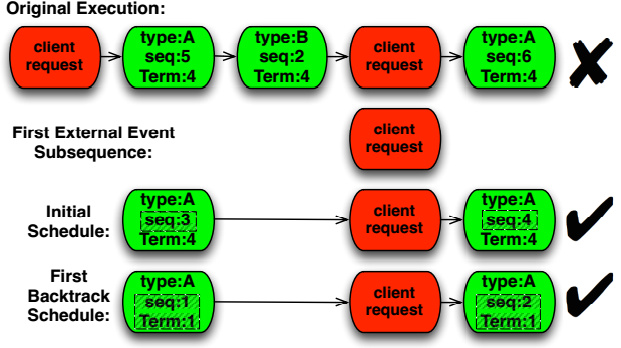
\includegraphics[width=2.5in]{./image/schedule.png}
\caption{Example schedules. External message deliveries are shown
in red, internal message deliveries in green.  The 'B' message becomes absent when exploring the first subsequence of external events. Initial schedule that is close to the original is chosen, except for the masked 'seq' field. The violation is not triggered after the initial schedule, so by matching messages by type, pending messages with smaller 'Term' numbers are delivered.}
\label{fig:schedule}
\setlength{\belowcaptionskip}{-3pt}
\end{figure}
\begin{table*}[t]
\caption{Overview of case studies. 'E:' is short for 'External Event'}
\label{tab:table1}
\centering
% centering table
\begin{tabular}{|c|c|c|c|c|c|c|}
\hline
Bug Name & Bug Type & Initial & Provenance & STSSched & TFB & Optimal\\
\hline
\hline
raft-45 &	Akka-FIFO, reproduced &	2160 (E:108)&	2138 (E:108)&	1183 (E:8) & 23 (E:8) & 22 (E:8)\\
\hline

raft-46 &	Akka-FIFO, reproduced &	1250 (E:108)&	1243 (E:108)&	674 (E:8) & 35 (E:8) & 23 (E:6)\\
\hline

raft-56 &	Akka-FIFO, found &	2380 (E:108)&	2376 (E:108)&	1427 (E:8) & 82 (E:8) & 21 (E:8)\\
\hline

raft-58a &	Akka-FIFO, found &	2850 (E:108)&	2824 (E:108)&	953 (E:32) & 226 (E:31) & 51 (E:11)\\
\hline

raft-58b &	Akka-FIFO, found &	1500 (E:208)&	1496 (E:208)&	164 (E:13) & 40 (E:8) & 28 (E:8)\\
\hline

raft-42 &	Akka-FIFO, reproduced &	1710 (E:208)&	1695 (E:208)&	1093 (E:39) & 180 (E:11) & 39 (E:16)\\
\hline

raft-66 &	Akka-UDP, found &	400 (E:68)&	392 (E:68)&	262 (E:23) & 77 (E:15) & 29 (E:10)\\
\hline

spark-2294 &	Akka-FIFO, reproduced &	1000 (E:30)&	886 (E:30)&	43 (E:3) & 40 (E:3) & 25 (E:1)\\
\hline

spark-3150 &	Akka-FIFO, reproduced &	600 (E:20)&	536 (E:20)&	18 (E:3) & 14 (E:3) & 11 (E:3)\\
\hline

spark-9256 &	Akka-FIFO, found &	300 (E:20)&	256 (E:20)&	11 (E:1) & 11 (E:1) & 11 (E:1)\\
\hline

\end{tabular}
\end{table*}

\textbf{Observation \#2: Data independence.} In \cite{9}, they observed that altered message contents such as differing sequence numbers do not affect the behavior of the program, meaning that the values of some message contents do not affect the system's control-flow. For matching messages, application developers give 'message fingerprint', which returns a string containing relevant parts of the message.  Fingerprint function might ignore sequence numbers and authentication cookies, but concatenate the other fields of messages.

\textbf{Observation \#3: Coarsen message matching.} It is desired to stay close to the original execution and not restrict to schedules that only match according to the user-defined message fingerprints from the original execution. This two goals can be achieved by considering a more coarse-grained match function: the type of pending messages. By 'type', we mean the language-level type tag of the message object, which is available to the RPC layer at runtime. Next schedules are explored by looking for pending messages whose types (not contents) match those in the original execution, in the exact same order that they appeared in the original execution. An example is depicted in Figure \ref{fig:schedule}.

\textbf{Observation \#4: Prioritize backtrack points that resolve match ambiguities. } When there are multiple pending messages that match, it initially only picks one. DPOR (eventually) sets backtrack points for all other co-enabled dependent events (regardless of type or message contents). There exists some small ambiguities in message contents as current execution is not completely identical to the original execution. Whenever it finds a backtrack point (pending message) that matches the type but not the fingerprint of an original delivery event from $\tau$, it replaces the original delivery with the backtrack's pending message, and execute the events before and after the backtrack point as before. In this way, it eventually explores all combinations of pending messages that match by type.


\textbf{Observation \#5: Shrink external message contents whenever possible. } The last observation is that the contents of the external messages should be minimized whenever possible because these messages can affect execution length. In akka-raft distributed system, initially the clusters (i.e., processes) do not know about their peers. Clusters instead wait to receive an external bootstrapping message that informs them of the identities of all other processes. The contents of the bootstrapping messages determine quorum size: how many acknowledgments are needed to reach consensus, and hence how many messages need to be delivered. If the application developer provides a function for separating the components of such message contents, then the algorithm  can minimize their contents by iteratively removing elements, and checking to see if the violation is still triggerable until no single remaining element can be removed.

\textbf{Minimizing internal events.} Once delta debugging over external events has completed, delta debugging is applied to internal events: for each subsequence of internal events chosen by delta debugging, the algorithm (i) marks those messages so that they are left pending and never delivered, and (ii) applies the same scheduling strategies described above for the remaining events to check whether the violation is still triggered.

\section{Experimental Results}
The experimental evaluation is totally focused by the minimization of the number of events produced by the DEMi tool. A high level overview of experimental findings are given in Table \ref{tab:table1}. The 'Bug Type' column shows two pieces of information: whether the bug can be triggered using TCP semantics (denoted as 'FIFO') or whether it can only be triggered when UDP is used; and whether the bug is  discovered while experimenting or whether the authors reproduced a known bug. The 'Provenance' column shows how many events from the initial execution remain after statically pruning events that are concurrent with the safety violation. The 'STSSched' column shows how many events remain after checking the initial schedules prescribed by the prior work of this tool by the same authors in \cite{3}  for each of delta debugging's subsequences. The 'TFB' column shows the final execution size after applying new proposed techniques ('Type Fingerprints with Backtracks'), where DPOR is directed to explore as many backtrack points that match the types of original messages (but no other backtrack points) as possible within the 12 hour time budget. Finally, the 'Optimal' column shows the size of the smallest violation-producing execution that is constructed by the authors by hand. The experiment is done on a 2.8GHz Westmere processor with 16GB memory.

Overall we can observe that DEMi produces executions that are within a factor of 1X to 4.6X (1.6X median) the size of the smallest possible execution that triggers that bug, and between 1X and 16X (4X median) smaller
than the executions produced by the previous technique (STSSched). STSSched is effective at minimizing external events (primary minimization target) for most case studies. TFB is significantly more effective for minimizing internal events (secondary target), especially for akka-raft. The tool is able to minimize almost 80\%-96\% reduction on the number of events. We can also observe that the minimization is not totally optimal, so there is some space for further improvement.

\section{Limitations}
\textbf{Safety vs. liveness.} This tool is primarily focused on safety violations, not liveness or performance bugs.

\textbf{Non-Atomic External Events.} DEMi currently waits for external events (e.g. crash-recoveries) to complete before proceeding. This may prevent it from finding bugs involving finer-grained event interleavings.

\textbf{Limited scale.} DEMi is currently tied to a single physical machine, which limits the scale of systems it can test. The common pitfalls in a distributed system: network overhead, message failures can incurred some scalability issues in DEMi; which is not observed yet.

\textbf{Shared memory \& disk.} In some systems processes communicate by writing to shared memory or disk rather
than sending messages over the network. Although DEMi do not currently support it, but it can be integrated by interposition to the runtime system as in \cite{10}, then DEMi would be able to treat writes to shared memory or disk in the same way it treats messages.

\section{Conclusions and Future Works}
Distributed systems are becoming more complex due to it's internal complexity. There exists many development tools to help for the development of sequential softwares. Observing the need to help in development of the distributed systems, DEMi tool is invented for minimization of the distributed executions. It has been proved to be a great tool to help the developers to fix development error in very short time and effort by empirical results. There are some spaces to enhance this tool. DEMi can be enhanced into more scalable system as well as capturing a wide range of distributed systems.







